\chapter{Research Questions and Analytical Framework}
\label{chap:framework}

\section{From a final prediction to a state trajectory}

For item $i$, let an architecture produce a sequence of observable stage texts
\begin{equation}
  T_i = \left(s_{i1}, s_{i2}, \ldots, s_{ik}, f_i\right),
\end{equation}
where $f_i$ is the final output and the preceding stages depend on the architecture. Each stage is mapped to two labels: discovery $D(s) \in \{\correct,\wrong,\uncertain\}$ and endorsement $E(s) \in \{\correct,\wrong,\uncertain\}$. The labels are defined relative to the reference answer and accepted aliases.

Discovery is \correct{} when the stage contains an answer-equivalent statement or enough explicit relational content to identify the answer. It is \wrong{} when this support is absent or supports a different answer. Endorsement is \correct{} when the answer-bearing statement commits to the reference answer, and \wrong{} when it commits elsewhere or explicitly rejects the reference answer. \uncertain{} is reserved for genuinely unresolvable cases, principally truncation inside the answer-bearing statement. The distinction is asymmetric: endorsement implies an answer decision, while discovery may be present in text that does not make a final commitment.

\begin{figure}[htbp]
  \centering
  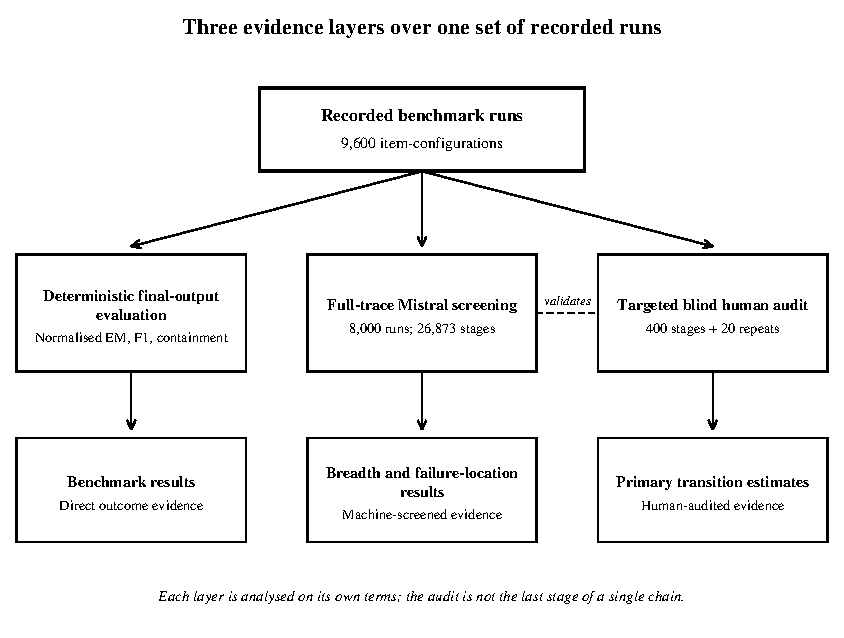
\includegraphics[width=0.96\textwidth]{figures/analysis_pipeline.pdf}
  \caption[Three evidence layers over the recorded runs]{Three evidence layers derived from the recorded benchmark runs. Deterministic final-output evaluation produces benchmark results; full-trace machine labels support breadth screening; and the blind human audit validates selected labels while independently supporting the primary Debate and Sequential transition estimates.}
  \label{fig:pipeline}
\end{figure}

\Cref{fig:pipeline} summarises three evidence layers derived from the recorded runs. Deterministic final-output evaluation produces benchmark results. Full-trace Mistral screening independently produces breadth and failure-location results. The targeted blind human audit both validates selected machine labels and supplies the primary transition estimates. The audit is therefore not merely the last transformation in a single scoring pipeline.

\section{Architecture-specific source states}

A universal definition of ``the previous stage'' would obscure the semantics of different computational graphs. Source states are therefore defined by the last point before the final coordination decision at which correctness can be meaningfully preserved.

For Debate, two agents first produce proposals and then revised answers after exposure to the opposing position. Let $r_{iA}$ and $r_{iB}$ be the revised outputs. The source endorsement is an oracle over these revisions:
\begin{equation}
  E_i^{\mathrm{src}} = \max\left(E(r_{iA}), E(r_{iB})\right),
\end{equation}
where the ordering is $\correct > \uncertain > \wrong$ for availability. The target is the final picker. This boundary measures whether the picker converts a correct revised option into the final answer. A separate machine-screened analysis examines proposal-to-revision changes, but the primary human transition estimate concerns the revision oracle to picker boundary.

For Sequential, workers receive the accumulated state in order. The source is the last worker output and the target is the final aggregator. This captures whether the aggregator preserves the chain's final answer state. Earlier worker transitions are useful diagnostics but are harder to interpret as homogeneous trials because workers may be assigned different subquestions.

For Parallel Roles and Ensemble, the natural source is the oracle over the candidate set and the target is the aggregator. For Subtask Parallel, candidate outputs are partial findings rather than complete answers, so oracle accuracy is not directly comparable with full-answer candidates. These three architectures remain in the benchmark and semantic screen, but are not included in the primary human transition audit.

\section{Outcome and transition metrics}

Final lexical performance is scored against the benchmark's own gold answer and its supplied aliases. The normalisation removes articles, punctuation, and redundant whitespace before comparison. Three comparison rules are used and are kept distinct throughout: normalised exact match, token-level F1, and normalised containment. \Cref{sec:lexical} defines all three formally and \Cref{tab:scoring-examples} gives worked examples of predictions that do and do not match under each. The headline benchmark figures in \Cref{chap:benchmark-results} use normalised containment and are named \emph{final normalised accuracy} there. Semantic metrics use the stage labels defined above.

For $N$ evaluated items, semantic discovery rate is
\begin{equation}
  \mathrm{DiscoveryRate} = \frac{1}{N}\sum_{i=1}^{N} \mathbb{I}\left[\exists s \in T_i : D(s)=\correct\right].
\end{equation}
Candidate-oracle accuracy restricts the maximum to the architecture's designated candidate stages. Final semantic accuracy is the proportion for which $D(f_i)=\correct$ under the screening protocol. Among items with a correct discovered state, preservation rate is
\begin{equation}
  \mathrm{Preservation} = P\left(D(f_i)=\correct \mid \exists s \in T_i : D(s)=\correct\right),
\end{equation}
and drop rate is its complement. Aggregation regret measures the difference between what the candidate set made available and what the system finally delivered,
\begin{equation}
  \mathrm{Regret} = \mathrm{OracleAccuracy} - \mathrm{FinalAccuracy},
  \label{eq:regret}
\end{equation}
where $\mathrm{OracleAccuracy}$ is the candidate-oracle accuracy defined above and $\mathrm{FinalAccuracy}$ is final semantic accuracy, both computed over the same $N$ items. A positive value indicates that the final decision failed to exploit available candidates. A negative value can occur for architectures such as Sequential or Subtask Parallel when aggregation synthesises partial evidence not individually sufficient for an oracle candidate label.

For the human analysis, the primary harmful and beneficial transition indicators are
\begin{align}
  H_i &= \mathbb{I}\left[E_i^{\mathrm{src}}=\correct \land E_i^{\mathrm{final}}=\wrong\right],\\
  B_i &= \mathbb{I}\left[E_i^{\mathrm{src}}=\wrong \land E_i^{\mathrm{final}}=\correct\right].
\end{align}
The rates $P(H_i=1)$ and $P(B_i=1)$ quantify damage and recovery at the final coordination boundary. Reporting both prevents a system with many destructive and many corrective changes from appearing equivalent to a stable system.

\section{Weighting the human audit}

The audit deliberately oversamples transitions that are rare in the full machine-screened population. Raw sample proportions therefore do not estimate population prevalence. Let $h$ index the frozen sampling strata, $N_h$ be the number of eligible items in a stratum, $n_h$ the audited sample, and $\bar{y}_h$ the audited transition rate. The finite-population weighted estimate is
\begin{equation}
  \hat{p} = \sum_h W_h\bar{y}_h, \qquad W_h = \frac{N_h}{\sum_h N_h}.
  \label{eq:weighting}
\end{equation}
An approximate stratified variance is
\begin{equation}
  \widehat{\mathrm{Var}}(\hat{p}) = \sum_h W_h^2\left(1-\frac{n_h}{N_h}\right)\frac{s_h^2}{n_h},
\end{equation}
where $s_h^2$ is the within-stratum sample variance. Intervals use $\hat{p} \pm 1.96\sqrt{\widehat{\mathrm{Var}}(\hat{p})}$ with bounds clipped to $[0,1]$. Because the final within-stratum selection also pursued coverage and balance, these intervals are descriptive approximations rather than confirmatory probability-sample intervals. The weighted point estimates are the primary summaries.

\section{Reliability thresholds and evidence hierarchy}

The project distinguishes three levels of evidence.

\begin{enumerate}[leftmargin=*]
  \item \textbf{Direct benchmark evidence}: exact match, F1, token use, truncation flags, and wall time are computed deterministically from recorded outputs and traces.
  \item \textbf{Machine-screened semantic evidence}: a Mistral judge labels all relevant stages. These data support broad patterns, candidate selection for audit, and descriptive failure localisation.
  \item \textbf{Human-audited transition evidence}: blinded human labels, hidden repeats, and frozen weights support the primary Debate and Sequential transition rates.
\end{enumerate}

This hierarchy follows from observed transfer failure. The judge performed strongly on a broad calibration set but materially worse on difficult transition-enriched examples. A second, stronger Qwen2.5-72B judge improved agreement but still failed the predetermined acceptance thresholds. Rather than selecting whichever machine result best supports a narrative, the analysis retains the human audit as controlling evidence and presents machine outputs with explicit caveats.

\section{Interpretive hypotheses}

The framework yields testable expectations without requiring a single global claim that MAS is good or bad. Architectures with independent candidates should have high discovery and oracle coverage. If their final accuracy is lower, the gap points to aggregation rather than exploration. Debate should show beneficial proposal-to-revision changes if cross-critique works as intended, but harmful changes if social conformity or persuasive errors dominate. Sequential workers should be vulnerable to state loss across the chain, while the final aggregator may recover from incomplete worker formulations. Larger budgets should improve outcomes if additional reasoning is productive; if they instead lengthen outputs, repeat information, or increase revision opportunities, discovery and preservation may stagnate or decline.

These hypotheses structure the results chapter. They are not all evaluated with the same evidential strength. Full-trace patterns generate architecture-level diagnoses, whereas the audited final-boundary estimates determine the main claim about Debate and Sequential preservation.
